\documentclass[12pt]{article}
\usepackage[utf8]{inputenc}

\usepackage[english, australian]{babel}
\usepackage[a4paper,left=20mm,right=20mm,top=20mm,bottom=20mm]{geometry}

\usepackage{tikz}
\usetikzlibrary{shapes.geometric, arrows, calc}
\tikzstyle{usr-file} = [rectangle, rounded corners, minimum width=3cm, minimum height=1cm,text centered, draw=black, text width=3cm]
\tikzstyle{code-file} = [rectangle, minimum width=3cm, minimum height=1cm, text centered, draw=black, text width=3cm]
\tikzstyle{arrow} = [thick,->,>=stealth]

\tikzset{
    between/.style args={#1 and #2}{
         at = ($(#1)!0.5!(#2)$)
    }
}

\usepackage{fancyhdr}
\pagestyle{fancy}

\title{ArmSim \\ \large Robotic Arm Simulator and Movement Programmer}
\author{Joshua Riddell \\ University of Queensland - 43947241}

\begin{document}
\maketitle

\section{Summary} % (fold)
\label{sec:summary}

Programming the complex movements of a robotic arm using direct angles and low level code is usually out of the scope of most factory operator's expertise, it is also a slow and tedious process for robot designers. ArmSim allows relatively quick and easy geometric definitions of robotic arms, and also provides a 3D representation of the arm. The 3D representation enables the user to program complex movements, and allow movement programming without the need for a physical arm to be present or built. ArmSim also includes a sequencer module - this allows the user to quickly prototype complex movement sequences.

% section summary (end)

\section{Topology Overview} % (fold)
\label{sec:topology_overview}

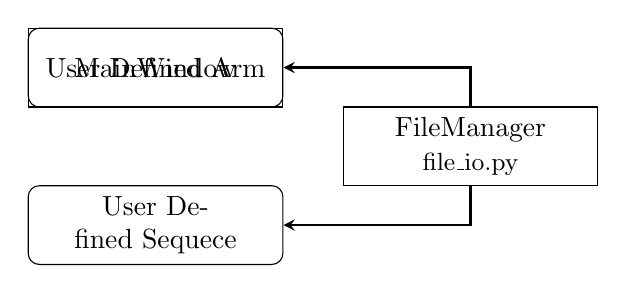
\begin{tikzpicture}[node distance=2cm]

% File reading end
\node (main) [code-file] {MainWindow};

\node (usr-arm) [usr-file] {User Defined Arm};
\node (usr-seq) [usr-file, below of=usr-arm] {User Defined Sequece};
\node (f-man) [code-file, between=usr-arm and usr-seq, xshift=4cm] {FileManager \\ \small file\_io.py};

\draw [arrow] (f-man) |- (usr-arm);
\draw [arrow] (f-man) |- (usr-seq);

% 




\end{tikzpicture}

% section topology_overview (end)

\end{document}